\chapter{Prerequisites}
\begin{chapquote}{H.G. Rice [1953], \textit{paraphrased by Anders Moller}}
  ``Everything interesting about the behaviour of programs is
  undecidable.''
\end{chapquote}

The goal of \textit{static program analysis} is to verify certain
\textsl{properties} (or \textsl{behaviours}, or
\textsl{specifications}, or \textsl{statements}, ...) of the target
program \textbf{without its execution}.

For program \textsl{P} and property \textsl{S},

\begin{itemize}
\item $ \SEM{P} $: Formal semantics of program \textsl{P}.

\item \textsl{S}: Semantic properties that we're interested in. This
  could be defined in various level, such as ``Division-by-zero will
  \textbf{never} occur'' or ``The variable \textit{i} is always 3''.

\item Soundness: $ analysis(P) = true \implies S $

\item Completeness: $ S \implies analysis(P) = true $

\item Scalability: Time complexity.
\end{itemize}


\textbf{No analysis} can be sound and complete at the same time. If an
analysis is sound, then it is also incomplete, and vice versa.

%%%%%%%%%%%%%%%%%%%%%%%%%%%%%%%%%%%%%%%%%%%%%%%%%%%%%%%%%%%%%%%%%%%%%%%%%%%%%%%%%%%%%%%%%%%%%%%%%%%%
\section{Relation Theory}
This note originates from
Proofwiki\footnote{https://proofwiki.org}.


\textbf{Relation theory} is the subfield of set theory concerned with
the properties of relations and relational structures. As a relation
has the same conceptual definition as a (graph-theoretical) graph, it
follows that there is considerable overlap between the fields of
relation theory and graph theory.

\subsection{Set Equivalence}

Let $S$ and $T$ be sets. Then $S$ and $T$ are \textbf{equivalent} if
and only if there exists a \textbf{bijection} $f : S \to T$ between
the elements of $S$ and those of $T$.

That is, if they have the \textbf{same cardinality}.

This can be written as $S \sim T$.

Other terms that are used that mean the same things as
\textbf{equivalent} are:

\begin{itemize}
\item \textbf{Equipotent}, from which we refer to equivalent sets as
  \textbf{having the same power}
\item \textbf{Equipollent}
\item \textbf{Equinumerous}
\item \textbf{Similar}
\end{itemize}

\subsection{Finite Set}

A set $S$ is defined as \textbf{finite} if and only if

\begin{math}
  \begin{array}{c}
    \exists n \in \mathbb{N}: S \sim \mathbb{N}_{< n}
  \end{array}
\end{math}

where $\sim$ denotes \textit{set equivalence}.

That is, if there exists an element $n$ of the set of natural numbers
$\mathbb{N}$ such that the set of all elements of $\mathbb{N}$ less
than $n$ is equivalent to $S$.

Equivalently, a finite set is a set with a count.



\subsection{Relation}
\subsubsection{Definition}
Let $S \times T$ be the Cartesian product of two sets $S$ and $T$.

A \textbf{relation} on $S \times T$ is an ordered triple
$ \mathcal{R} = (S, T, R) $ where $R \subseteq S \times T$ is a
subset of the Cartesian product of $S$ and $T$.

What this means is that a \textbf{relation} \textit{relates} (certain)
elements of one set or class $S$ with (certain) elements of another,
$T$. Not all elements of $S$ need to be related to every (or even any)
element of $T$.

\subsubsection{Notation}

If $(x, y)$ is an ordered pair such that $(x, y) \in \mathcal{R}$, we
use the notation: $ s \mathcal{R} t$ or $ \mathcal{R}(s, t)$ and can
say:
\begin{itemize}
\item $s$ bears $\mathcal{R}$ to $t$
\item $s$ stands in the relation $\mathcal{R}$ to $t$
\end{itemize}

\subsubsection{General Definition}
Let
$\mathbb{S} = \Pi^n_{i=1}S_i = S_1 \times S_2 \times ... \times S_n $
be the Cartesian product on $n$ sets $S_1, ..., S_n$.

An \textbf{$n$-ary relation on} $\mathbb{S}$ is an ordered
$n+1$-tuple $\mathcal{R}$ defined as
$\mathcal{R} := (S_1, S_2, ..., S_n, R)$, where $R$ is an arbitrary
subset $R \subseteq \mathbb{S}$.

To indicate that $(s_1, s_2, ..., s_n) \in R$, we
write: $\mathcal{R}(s_1, s_2, ..., s_n)$

\subsubsection{Unary Relation}
As a special case of an $n$-ary relation on $S$, note that when $n=1$
we define a \textbf{unary relation} on $S$ as
$\mathcal{R} \subseteq S$. That is, a \textbf{unary relation} is a
subset of $S$.

\subsubsection{Endorelation}
Let $S \times S$ be the Cartesian product of a set or class $S$ with
itself. Let $\mathcal{R}$ be a \textbf{relation} on $S \times S$. Then
$\mathcal{R}$ is referred to as an \textbf{endorelation on} $S$.


The term \textbf{endorelation} is rarely seen. Once it is established
that the \textit{domain and codomain of a given relation are the same
  set}, further comment is rarely needed.


An \textbf{endorelation} is also called a \textbf{relation in} $S$, or
a \textbf{relation on} $S$. The latter term is discouraged, though,
because it can also mean a left-total relation, and confusion can
arise.

Some sources use the term \textbf{binary relation} exclusively to
refer to a \textbf{binary endorelation}.


\subsection{Symmetry}
\label{sec:symmetry}
The word \textit{symmetry} comes from Greek symmetria meaning
\textbf{measure together}.

\subsubsection{Definition}

Let $\mathcal{R} \subseteq S \times S$ be a relation in $S$.



\paragraph{Symmetric}

$\mathcal{R}$ is \textbf{symmetric} if and only if
$(x, y) \in \mathcal{R} \implies (y, x) \in \mathcal{R}$.

\paragraph{Asymmetric}

$\mathcal{R}$ is \textbf{asymmetric} if and only if
$(x, y) \in \mathcal{R} \implies (y, x) \notin \mathcal{R}$.

\paragraph{Antisymmetric}

$\mathcal{R}$ is \textbf{antisymmetric} if and only if
$ (x,y) \in \mathcal{R} \land (y, x) \in \mathcal{R} \implies x = y $.
That is, $\{(x, y), (y, x) \} \subseteq \mathcal{R} \implies x = y $.

\paragraph{Non-symmetric}

$\mathcal{R}$ is \textbf{non-symmetric} if and only if it is neither
\textit{symmetric} nor \textit{asymmetric}.

\subsubsection{Antisymmetric and Asymmetric}

Note the difference between:
\begin{itemize}
\item An \textit{asymmetric relation}, in which the fact that
  $(x, y) \in \mathcal{R}$ means that $(y, x)$ is defintely
  \textbf{not} in $\mathcal{R}$
\item An \textit{antisymmetric relation}, in which there \textit{may}
  be instances of both $(x, y) \in \mathcal{R}$ and
  $(y, x) \in \mathcal{R}$, but if there are, then it means that $x$
  and $y$ have to be the same object.
\end{itemize}


\subsection{Reflexivity}
\label{sec:reflexivity}

\subsubsection{Definition}

Let $\mathcal{R} \subseteq S \times S$ be a relation in $S$.

\paragraph{Reflexive}

$\mathcal{R}$ is \textbf{reflexive} if and only if
$ \forall x \in S : (x, x) \in \mathcal{R} $.

\paragraph{Coreflexive}

$\mathcal{R}$ is \textbf{coreflexive} if and only if
$ \forall x, y \in S : (x, y) \in \mathcal{R} \implies x = y$.

\paragraph{Antireflexive}

$\mathcal{R}$ is \textbf{antireflexive} if and only if
$ \forall x \in S: (x, x) \notin \mathcal{R}$.

\paragraph{Non-reflexive}

$\mathcal{R}$ is \textbf{non-reflexive} if and only if it is neither
\textit{reflexive} nor \textit{antireflexive}.


\subsection{Transitivity}
\label{sec:transitivity}

\subsubsection{Definition}

Let $\mathcal{R} \subseteq S \times S$ be a relation in $S$.

\paragraph{Transitive}

$\mathcal{R}$ is \textbf{transitive} if and only if
$(x, y) \in \mathcal{R} \land (y, z) \in \mathcal{R} \implies (x, z)
\in \mathcal{R}$. That is,
$\{(x, y), (y, z)\} \subseteq \mathcal{R} \implies (x, z) \in
\mathcal{R}$.

\paragraph{Antitransitive}

$\mathcal{R}$ is \textbf{antitransitive} if and only if
$ (x, y) \in \mathcal{R} \land (y, z) \in \mathcal{R} \implies (x, z)
\notin \mathcal{R}$. That is,
$ \{ (x, y), (y, z) \} \subseteq \mathcal{R} \implies (x, z) \notin
\mathcal{R} $.

\paragraph{Non-transitive}

$\mathcal{R}$ is \textbf{non-transitive} if and only if it is neither
\textit{transitive} nor \textit{antitransitive}.


\subsection{Total Relation}
\label{sec:total-relation}
Let $\mathcal{R} \subseteq S \times S$ be a relation on a set
$S$. Then $\mathcal{R}$ is defined as \textbf{total} if and only if:

$\forall a, b \in S : (a, b) \in \mathcal{R} \lor (b, a) \in
\mathcal{R}$

That is, if and only if every pair of elements is related.


Also called as \textbf{strictly connected}, or \textbf{complete
  relation}.

\subsection{Connected Relation}
\label{sec:connected-relation}

Let $\mathcal{R} \subseteq S \times S$ be a relation on a set
$S$. Then $\mathcal{R}$ is \textbf{connected} if and only if:

$\forall a, b \in S: a \neq b \implies (a, b) \in \mathcal{R} \lor
(b,a) \in \mathcal{R}$

That is, if and only if every pair of \textit{distinct} elements is
related.


Also called as \textbf{weakly connected}, while \textit{strictly
  connected} refers to \textit{total relation}.


%%%%%%%%%%%%%%%%%%%%%%%%%%%%%%%%%%%%%%%%%%%%%%%%%%%%%%%%%%%%%%%%%%%%%%%%%%%%%%%%%%%%%%%%%%%%%%%%%%%
\section{Ordering}
\label{sec:ordering}

\paragraph{Definition}

Let $S$ be a set.

An \textbf{ordering on} $S$ is a relation $\mathcal{R}$ on $S$ such
that:

\begin{itemize}
\item $\mathcal{R}$ is \textbf{reflexive}, i.e., $\forall a \in S: a \mathcal{R} a$.
\item $\mathcal{R}$ is \textbf{transitive}, i.e.,
  $\forall a, b, c \in S: a \mathcal{R} b \land b \mathcal{R} c
  \implies a \mathcal{R} c$.
\item $\mathcal{R}$ is \textbf{antisymmetric}, i.e.,
  $\forall a \in S : a \mathcal{R} b \land b \mathcal{R} a \implies a
  = b$.
\end{itemize}

It is not demanded for an ordering $\preceq$, defined in its most
general form on a set $S$, that \textit{every} pair of elements of $S$
is related by $\preceq$. They may be, or they may not be, depending on
the specific nature of both $S$ and $\preceq$.

If it \textit{is} the case that $\preceq$ is a \textbf{connected
  relation}, that is, that every pair of distinct elements is related
by $\preceq$, then $\preceq$ is called a \textbf{total ordering}.

If it is \textit{not} the case that $\preceq$ is connected, then
$\preceq$ is called a \textbf{partial ordering}.


\paragraph{Notation}

Symbols used to denote a general \textbf{ordering relation} are
usually variants on $\preceq$, $\leq$, and so on.

Thus, $a \preceq b$ can be read as:
\begin{itemize}
\item $a$ \textbf{precedes, or is the same as} $b$.
\item $b$ \textbf{succeeds, or is the same as} $a$.
\end{itemize}

\paragraph{Smaller and Larger}

An \textbf{ordering} can often be considered to be a comparison of the
\textbf{size} of objects, perhaps in some intuitive sense. This is
particularly applicable in the context of numbers. Thus the expression
$A \preceq B$ can in such contexts be interpreted as:
\begin{itemize}
\item $A$ is \textbf{smaller than} $B$
\item $A$ is \textbf{less than} $B$
\item $B$ is \textbf{larger than} $A$
\item $B$ is \textbf{greater than} $A$
\end{itemize}

In natural language, such terms are called \textbf{comparative
  adjectives}, or just \textbf{comparatives}.

Depending on the nature of the set being ordered, and depending on the
nature of the ordering relation, this interpretation of an ordering as
a comparison of size may not be intellectually sustainable.

\subsection{Upper Bound}
Let $(S, \preceq)$ be an ordered set. Let $T \subseteq S$.

An \textbf{upper bound for $T$ in $S$} is an element $M \in S$ such
that:

\begin{math}
  \begin{array}{c}
    \forall t \in T : t \preceq M
  \end{array}
\end{math}

That is, $M$ \textit{succeeds} every elements of $T$.



\subsection{Supremum}

Let $(S, \preceq)$ be an ordered set. Let $T \subseteq S$.

An element $c \in S$ is the \textbf{supremum of $T$ in $S$} if and
only if:

\begin{itemize}
\item $c$ is an \textit{upper bound} of $T$ in $S$
\item $c \preceq d$ for all upper bounds $d$ of $T$ in $S$
\end{itemize}

If there exists a \textbf{supremum} of $T$, we say that:

\begin{itemize}
\item $T$ admits a supremum (in $S$)
\item $T$ has a supremum (in $S$)
\end{itemize}


Particularly in the field of analysis, the supremum of a set $T$ is
often referred to as the \textbf{least upper bound of $T$} and denoted
$\mathtt{lub}(T)$.


\subsubsection{Supremum is Unique}

$T$ has at most one supremum in $S$.

\paragraph{Proof}

Let $c$ and $c'$ both be suprema of $T$ in $S$. From the definition of
supremum, $c$ and $c'$ are upper bounds of $T$ in $S$.

By that definition:

\begin{itemize}
\item $c$ is an upper bound of $T$ in $S$, and $c'$ is a supremum of $T$ in $S$ implies that $c' \preceq c$.
\item $c'$ is an upper bound of $T$ in $S$, and $c$ is supremum of $T$ in $S$ implies that $c preceq c'$.
\end{itemize}


So

\begin{math}
  \begin{array}{c}
    c' \preceq c \land c \preceq c'
  \end{array}
\end{math}

and thus by the antisymmetry of the ordering $\preceq$:

\begin{math}
  \begin{array}{c}
    c = c' \\
  \end{array}
\end{math}

Q.E.D.


\subsection{Join}
Let $(S, \preceq)$ be an ordered set. Let $a, b \in S$. Let their
supremum $\mathtt{sup} \{a, b\}$ exist in $S$.

Then the \textbf{join of $a$ and $b$}\footnote{some sources refer to
  this as the \textbf{union} of $a$ and $b$} is defined as:

\begin{math}
  \begin{array}{c}
    a \vee b = \mathtt{sub} \{ a, b \}
  \end{array}
\end{math}

Expanding the definition of supremum, one sees that $c = a \vee b$ if
and only if:

\begin{math}
  \begin{array}{c}
    a \preceq c\text{ and }b \preceq c\text{ and }\forall s \in S: a \preceq s \land b \preceq s \implies c \preceq s
  \end{array}
\end{math}



\subsection{Lower Bound}
Let $(S, \preceq)$ be an ordered set. Let $T \subseteq S$.

A \textbf{lower bound for $T$ in $S$} is an element $m \in S$ such that:

\begin{math}
  \begin{array}{c}
    \forall t \in T: m \preceq t
  \end{array}
\end{math}

That is, $m$ \textit{precedes} every elements of $T$.


\subsection{Infimum}
Let $(S, \preceq)$ be an ordered set. Let $T \subseteq S$.


An element $c \in S$ is the \textbf{infimum of $T$ in $S$} if and only
if:

\begin{itemize}
\item $c$ is a \textit{lower bound} of $T$ in $S$
\item $d \preceq c$ for all lower bounds $d$ of $T$ in $S$
\end{itemize}

If there exists an \textbf{infimum} of $T$, we say that:

\begin{itemize}
\item $T$ admits an infimum (in $S$)
\item $T$ has an infimum (in $S$)
\end{itemize}


Particularly in the field of analysis, the infimum of a set $T$ is
often referred to as the \textbf{greatest lower bound of $T$} and
denoted as $\mathtt{glb}(T)$.


\subsection{Meet}
Let $(S, \preceq)$ be an ordered set. Let $a, b \in S$. Let their
infimum $\mathtt{inf} \{a, b\}$ exist in $S$.

Then the \textbf{meet of $a$ and $b$}\footnote{some sources refer to
  this as the \textbf{intersection} of $a$ and $b$} is defined as:

\begin{math}
  \begin{array}{c}
    a \wedge b =\mathtt{inf} \{ a, b \}
  \end{array}
\end{math}


Expanding the definition of infimum, one sees that $c = a \wedge b$ if
and only if:

\begin{math}
  \begin{array}{c}
    c \preceq c\text{ and }c \preceq b\text{ and } \forall s \in S: s \preceq a \land s \preceq b \implies s \preceq c
  \end{array}
\end{math}



\subsection{Well-Ordering}

Let $(S, \preceq)$ be an ordered set.

The ordering $\preceq$ is a \textbf{well-ordering} on $S$ if and only
if \textbf{every} non-empty subset of $S$ has a smallest element under
$\preceq$. That is,


\begin{math}
  \begin{array}{c}
    \forall T \subseteq S: \exists a \in T : \forall x \in T : a \preceq
    x
  \end{array}
\end{math}

\subsection{Strict Ordering}
\label{sec:strict-ordering}

Let $\mathcal{R}$ be a relation on a set $S$.

Then $\mathcal{R}$ is a \textbf{strict ordering} on $S$ if and only
if:

\begin{itemize}
\item $\mathcal{R}$ is \textit{asymmetric}, i.e.,
  $\forall a, b \in S : a \mathcal{R} b \implies \neg b \mathcal{R} a$
\item $\mathcal{R}$ is \textit{transitive}, i.e.,
  $\forall a, b, c \in S: a \mathcal{R} b \land b \mathcal{R} c
  \implies a \mathcal{R} c$
\end{itemize}

Symbols used to denote a general strict ordering are usually variants
on $\prec$, $<$, and so on.


\subsection{Total Ordering}

Let $\mathcal{R} \subseteq S \times S$ be a relation on a set $S$.

$\mathcal{R}$ is a \textbf{total ordering} on $S$ if and only if:

\begin{itemize}
\item $\mathcal{R}$ is an ordering on $S$
\item $\mathcal{R}$ is connected
\end{itemize}

That is, $\mathcal{R}$ is an ordering with no non-comparable pairs:


\begin{math}
  \begin{array}{c}
    \forall x, y \in S: x \mathcal{R} y \lor y \mathcal{R} x
  \end{array}
\end{math}

Also called as a \textbf{linear ordering}, or a \textbf{simple
  ordering}.

If it is necessary to emphasises that a total ordering is \textbf{not}
strict, then the term \textbf{weak total ordering} may be used.


\subsection{Partial Ordering}

Let $(S, \preceq)$ be an ordered set.

Then the ordering $\preceq$ is a \textbf{partial ordering} on $S$ if
and only if $\preceq$ is \textbf{not connected}.

That is, if and only if $(S, \preceq)$ has at least one pair which is
non-comparable:

\begin{math}
  \begin{array}{c}
    \exists x, y \in S : x \npreceq y \land y \npreceq x
  \end{array}
\end{math}


It it is necessary to emphasizes that a partial ordering is
\textbf{not} strict, then the term \textbf{weak partial ordering} may
be used.


%%%%%%%%%%%%%%%%%%%%%%%%%%%%%%%%%%%%%%%%%%%%%%%%%%%%%%%%%%%%%%%%%%%%%%%%%%%%%%%%%%%%%%%%%%%%%%%%%%%%%%%%%%%%%%%%%%
\section{Soundness and Completeness}

\subsection{Soundness}


It is called \textbf{sound} if an analysis for program \textsl{P} says
that it satisfies property \textsl{S}, then the program will truly
satisfy that property.

\textbf{Sound} but \textbf{incomplete} analysis have \textbf{false
  positive}. In other words, it does \textbf{not prove} programs that
satisfy the property.

\begin{figure}[h]
  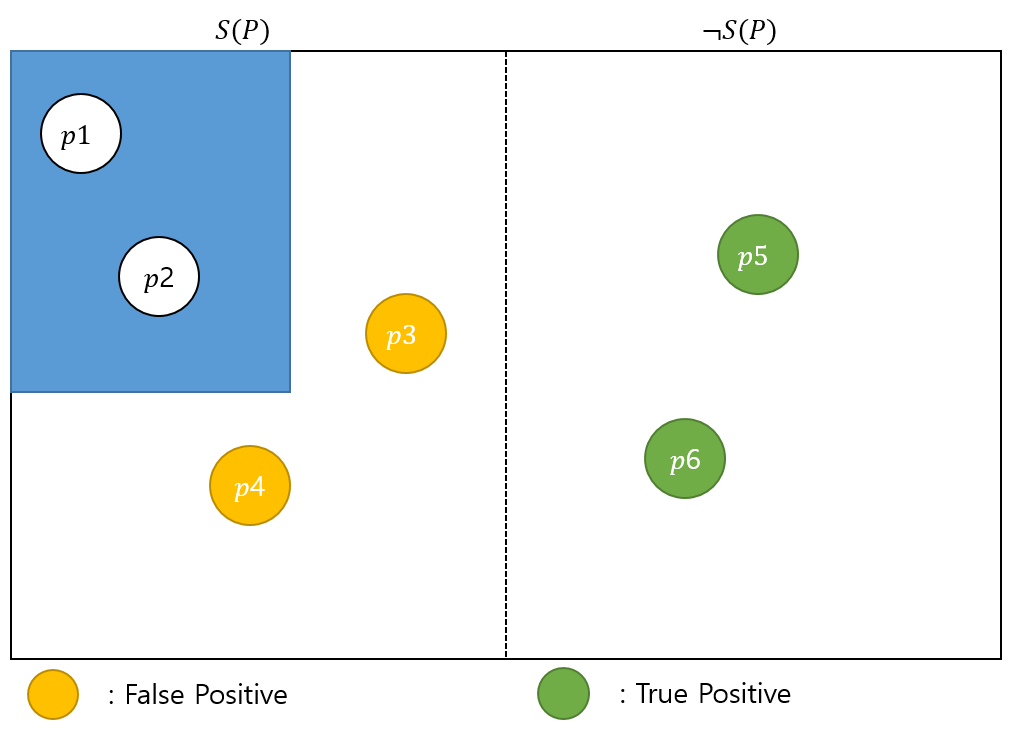
\includegraphics[width=\textwidth]{sound}
  \caption{Sound Analysis}
  \label{fig:sound}
\end{figure}

Figure \ref{fig:sound} shows a sound analysis (the blue area). It
proves correctly for the programs $ p_1 $ and $ p_2 $ that satisfy the
specification ($S(P)$). However, since this analysis is
\textit{incomplete}, it has \textbf{false positives}: it \textbf{does
  not prove} for programs $ p_3 $ and $ p_4 $ that satisfy $S$. In
other words, it proves that $ p_3 $ and $ p_4 $ satisfy $ \neg S(P) $
by emiting \textbf{alarms}, even though they are actually satisfy
$ S(P) $. False positives are also called as \textbf{false alarms}.

\subsection{Completeness}

An analysis is called \textbf{complete} when a program satisfies a
property \textsl{S}, the analysis for that program says that it will
satisfy that property.


\textbf{Complete} but \textbf{unsound} analysis have \textbf{false
  negative}. In other words, it \textbf{wrongly proves} programs that
does not satisfy the property.


\begin{figure}[h]
  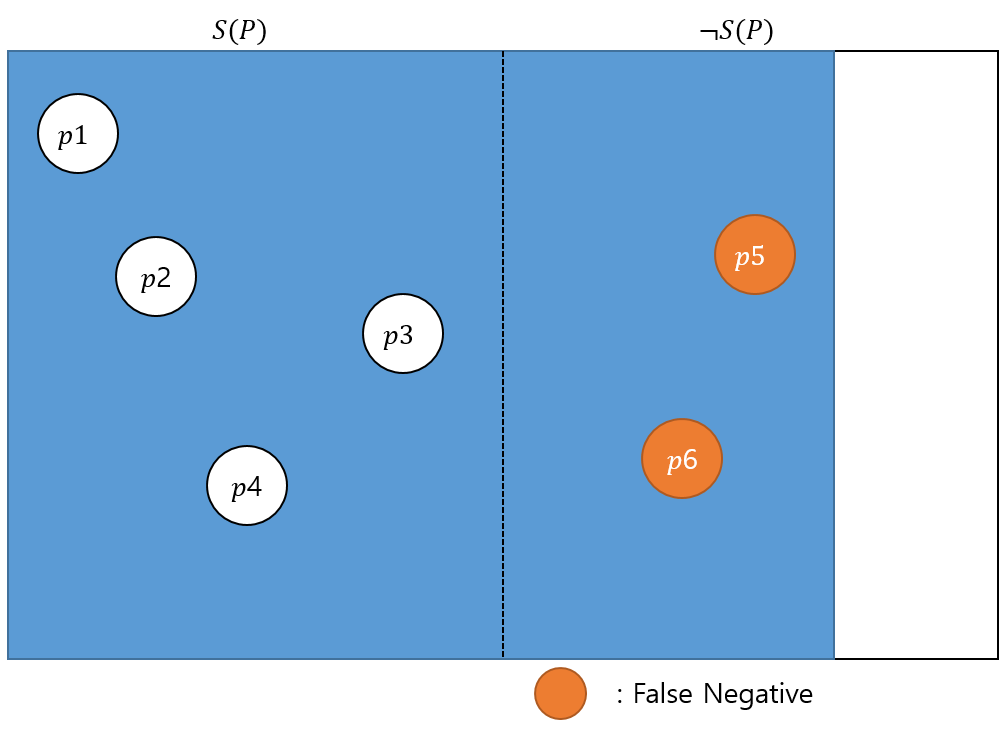
\includegraphics[width=\textwidth]{complete}
  \caption{Complete Analysis}
  \label{fig:complete}
\end{figure}

Figure \ref{fig:complete} shows a complete analysis (also the blue
area). It proves all the programs. In other words, it \textbf{wrongly
  proves} for programs $ p_5 $ and $ p_6 $ that actually do not
satisfy $ S(P) $ by accepting those programs (i.e., emitting no
alarms), thus it is \textit{unsound}. Those programs are \textbf{false
  negatives}.


The table \ref{tab:summary} shows the summary of soundness and
completeness.

\begin{table}[ht]
  \centering
  \caption{Sound \& Complete Summary}
  \label{tab:summary}

  \begin{tabular}[t]{l>{\raggedright}p{0.3\linewidth}>{\raggedright\arraybackslash}p{0.3\linewidth}}
    \hline
    & $ S(P) $ & $ \neg S(P) $ \\
    \hline
    Prove \texttt{(accept)} & \textbf{True negative} (\textsl{correct inference}) & False negative \\
    Not prove \texttt{(reject, alarm)} & False positive & \textbf{True positive} (\textsl{correct inference}) \\
    \hline
  \end{tabular}
\end{table}%



%%%%%%%%%%%%%%%%%%%%%%%%%%%%%%%%%%%%%%%%%%%%%%%%%%%%%%%%%%%%%%%%%%%%%%%%%%%%%%%%%%%%%%%%%%%%%%%%%%%%%%%%%%%%%%%%%%
\section{Semantics of Program}
\label{sec:semantics}

Semantics of the program defines the \textbf{meaning} of the program
that is grammatically correct.

\subsection{Prerequisites}

\subsubsection{Simple Language Syntax}

\begin{math}
  \begin{array}{llll}
    a \to & \mid n & \mid x & \mid a_1 + a_2 \\
          & \mid a_1 \times a_2 & \mid a_1 - a_2 \\
    b \to & \mid \mathtt{true} & \mid \mathtt{false} & \mid a_1 = a_2  \\
          & \mid a_1 \leq a_2 & \mid \neg b & \mid b_1 \land b_2 \\
    c \to & \mid x := a  & \mid \mathtt{skip} & \mid c_1 ; c_2 \\
          & \mid \mathtt{if} \text{ }b \text{ }c_1\text{ }c_2 & \mid \mathtt{while} \text{ }b \text{ }c \\
  \end{array}
\end{math}

A state $ s \in State $ is a function from variables to values:
\begin{math}
  \begin{array}{rcl}
    State & : & Var \to \mathbb{Z} \\
  \end{array}
\end{math}


\subsubsection{Semantics of Arithmetic Expressions}

\begin{math}
  \begin{array}{rcl}
    \mathcal{A} & : & \mathtt{Aexp} \to State \to \mathbb{Z} \\
    \mathcal{A} \SEM{ a } & : & State \to \mathbb{Z} \\
    \mathcal{A} \SEM{ n } (s) & = & n \\
    \mathcal{A} \SEM{ x } (s) & = & s(x) \\
    \mathcal{A} \SEM{ a_1 + a_2 } (s) & = & \mathcal{A} \SEM{ a_1 } (s) + \mathcal{A} \SEM{ a_2 } (s) \\
    \mathcal{A} \SEM{ a_1 \times a_2 } (s) & = & \mathcal{A} \SEM{ a_1 } (s) \times \mathcal{A} \SEM{ a_2 } (s) \\
    \mathcal{A} \SEM{ a_1 - a_2 } (s) & = & \mathcal{A} \SEM{ a_1 } (s) - \mathcal{A} \SEM{ a_2 } (s) \\
  \end{array}
\end{math}

\subsubsection{Semantics of Boolean Expressions}

\begin{math}
  \begin{array}{rcl}
    \mathcal{B} & : & \mathtt{Bexp} \to State \to {T} \\
    {T} & = & \{ {true}, {false} \} \\
    \mathcal{B} \SEM{ b } & : & State \to {T} \\
    \mathcal{B} \SEM{ \mathtt{true} } (s) & = & {true} \\
    \mathcal{B} \SEM{ \mathtt{false} } (s) & = & {false} \\
    \mathcal{B} \SEM{ a_1 = a_2 } (s) & = & \mathcal{A} \SEM{ a_1 } (s) = \mathcal{A} \SEM{ a_2 } (s) \\
    \mathcal{B} \SEM{ a_1 \leq a_2 } (s) & = & \mathcal{A} \SEM{ a_1 } (s) \leq \mathcal{A} \SEM{ a_2 } (s) \\
    \mathcal{B} \SEM{ \neg b } (s) & = & \mathcal{B} \SEM{ b } (s) = {false} \\
    \mathcal{B} \SEM{ b_1 \land b_2 } (s) & = & \mathcal{B} \SEM{ b_1 } (s) \wedge \mathcal{B} \SEM{ b_2 } (s) \\
  \end{array}
\end{math}

\subsubsection{Free Variables}

A set of variables occurring in the expression.

\begin{math}
  \begin{array}{rcl}
    FV(n) & = & \emptyset \\
    FV(x) & = & \{ x \} \\
    FV(a_1 + a_2) & = & FV(a_1) \cup FV(a_2) \\
    FV(a_1 \times a_2) & = & FV(a_1) \cup FV(a_2) \\
    FV(a_1 - a_2) & = & FV(a_1) \cup FV(a_2) \\
  \end{array}
\end{math}

q\paragraph{Lemma}

Let $ s $ and $ s' $ be two states satisfying that $ s(x) = s'(x) $
for all $ x \in FV(a) $.

Then, $ \mathcal{A} \SEM{ a } (s) =\mathcal{A} \SEM{ a } (s') $ holds.

\paragraph{Lemma}

Let $ s $ and $ s' $ be two states satisrying that $ s(x) = s'(x) $
for all $ x \in FV(b) $.

Then, $ \mathcal{B} \SEM{ b } (s) = \mathcal{B} \SEM{ b } (s') $
holds.


\subsubsection{Substitution}

$ a [ y \mapsto a_0 ] $ means the arithmetic expression obtained by
replacing each occurrence of $ y $ in $a $ by $ a_0 $.

\begin{math}
  \begin{array}{rcl}
    n[y \mapsto a_0 ] & = & n \\
    x[y \mapsto a_0 ] & = & \begin{cases}
      a_0 & \mathtt{if} x = y \\
      x & \mathtt{if} x \neq y \\
    \end{cases} \\
    (a_1 + a_2)[y \mapsto a_0] & = & (a_1[y \mapsto a_0]) + (a_2[y \mapsto a_0]) \\
    (a_1 \times a_2)[y \mapsto a_0] & = & (a_1[y \mapsto a_0]) \times (a_2[y \mapsto a_0]) \\
    (a_1 - a_2)[y \mapsto a_0] & = & (a_1[y \mapsto a_0]) - (a_2[y \mapsto a_0]) \\
  \end{array}
\end{math}


\begin{math}
  (s[y \mapsto v])(x) =
  \begin{cases}
    v & \mathtt{if} x = y \\
    s(x) & \mathtt{if} x \neq y \\
  \end{cases}
\end{math}



\paragraph{Lemma}
$\mathcal{A} \SEM{ a[y \mapsto a_0] } (s) = \mathcal{A} \SEM{a} (s [ y
\mapsto \mathcal{A} \SEM{a_0} (s)]) $ for alll state s.



%%%%%%%%%%%%%%%%%%%%%%%%%%%%%%%%%%%%%%%%%%%%%%%%%%%%%%%%%%%%%%%%%%%%%%%%%%%%%%%%%%%%%%%%%%%%%%%%%%%%%%%%%%%%%%%%%%
\subsection{Operational Semantics}

Also called as \textit{transitional} semantics.

Semantics of a program is defined by the computation steps executed on
a machine. In other words, operational semantics is concerned about
\textbf{how to execute} the program and not merly what the execution
result is.

The semantics is defined as a transition system
$ ( \mathbb{S}, \to ) $, where

\begin{itemize}
\item $ \mathbb{S} $ is the set of all \textbf{possible states}.
\item $ \to \subseteq \mathbb{S} \times \mathbb{S} $ is a
  \textbf{transition relation} between two states. Describes how the
  execution takes place.
\item $ s \in \mathbb{S} $ is a \textbf{state} of the program. It is
  either $ \pair{ S, s }$ which is a non-terminal state (i.e., the
  statement $ S $ is to be executed from the state $ s $), or $ s $
  which is a terminal state.
\end{itemize}

There are two approaches for operational semantics.  The difference
between the two are in the definitions of \textsl{transition
  relation}.

\subsubsection{Big-step}
\label{sec:big-step}

Big-step operational semantics describes how the \textbf{overall
  results} of executions are obtained.

The transition relation specified the relationship between the initial
state and the final state: $ \pair{ S, s } \to s' $

Transition relation is defined with \textbf{inference rules} of the
form:
\\

\begin{math}
\frac{ \pair{ S_1, s_1} \to s_1', ..., \pair{ S_n, s_n} \to s_n' }
{ \pair{S, s} \to s' }
\text{ if ... }
\end{math}

where

\begin{itemize}
\item $ S_1, ..., S_n $ are \textsl{statements} that consistute $ S $.
\item A rule has a number of premises and one conclusion.
\item A rule may also have a number of conditions that have to be
  fulfilled whenever the rule is applied.
\item Rules without premises are called \textbf{axioms}.
\end{itemize}

Big-step operational semantics for the while language is:


\begin{tabularx}{\textwidth}{c}
\\
$ \overline{ \pair{ x := a, s } \to s [ x \mapsto \mathcal{A}\SEM{a}(s) ] } $\\
\\
$ \overline{ \pair{ \mathtt{skip}, s} \to s } $\\
\\

$ \underline{ \pair{S_1, s} \to s' \text{   } \pair{S_2, s'} \to s''} $ \\
$ \pair{S_1;S_2, s} \to s'' $ \\
\\

\end{tabularx}


\paragraph{Semantic Function for Statements}

The \textbf{semantic function} for statements is the partial function:

\begin{math}
  \begin{array}{rcl}
    \mathcal{S}_b & : & Stm \to ( State \to State) \\
    \mathcal{S}_b \SEM{S} (s) & = &
                                    \begin{cases}
                                      s' & \mathtt{if} \pair{S, s} \to s' \\
                                      \mathbf{undef} & \mathtt{otherwise}
                                    \end{cases}

  \end{array}
\end{math}


\subsubsection{Small-step}
\label{sec:small-step}

Small-step operational semantics describes how the \textbf{individual
  steps} of the computations take place.

The individual computation steps are described by the transition
relation of the form:
\\

\begin{math}
  \pair{S, s} \implies \gamma
\end{math}

where $\gamma$ is either non-terminal state or terminal state. The
transition expresses the first step of the execution of $S$ from state
$s$.

\begin{itemize}
\item If $ \gamma = \pair{S', s'} $, non-terminal state, then the
  execution of $S$ from $s$ is not completed and the remaining
  computation continues with $\pair{S', s'}$.
\item If $ \gamma = s'$, terminal state, then the execution of $S$
  from $s$ has terminated and the final state is $s'$.
\end{itemize}

We say $\pair{S, s}$ is \textbf{stuck} if there is no $\gamma$ such
that $\pair{S, s} \implies \gamma$.

\paragraph{Semantic Function}

The semantic function $\mathcal{S}_s$ for small-step semantics is:
\begin{math}
  \begin{array}{rcl}
    \mathcal{S}_s & : & Stm \to (State \to State) \\
    \mathcal{S}_s \SEM{S} (s) & = &
                                    \begin{cases}
                                      s' & \mathtt{if} \pair{S, s} \xRightarrow{*} s' \\
                                      \mathbf{undef} & \mathtt{otherwise}
                                    \end{cases}

  \end{array}
\end{math}


%%%%%%%%%%%%%%%%%%%%%%%%%%%%%%%%%%%%%%%%%%%%%%%%%%%%%%%%%%%%%%%%%%%%%%%%%%%%%%%%%%%%%%%%%%%%%%%%%%%%%%%%%%%%%%%%%%
\subsection{Denotational Semantics}
Also called as \textit{compositional} semantics.

Semantics of a program is defined by the semantics of the sub-parts of
the program. Thus, proving its soundness is by structural induction on
the program. For some realistic programming languages, even defining
their compositional semantics is an obstacle, due to \texttt{goto},
\texttt{exception}, or \texttt{call}.


%%% Local Variables:
%%% mode: latex
%%% TeX-master: "program-analysis"
%%% End:
